\begin{anexosenv}

\partanexos

\chapter{Protótipo de Alta Fidelidade}
\label{protot}

Segue-se a representação do protótipo de alta fidelidade do aplicativo descrito em na seção \ref{sec:prot}.

\begin{figure}[!h]
  \centering
  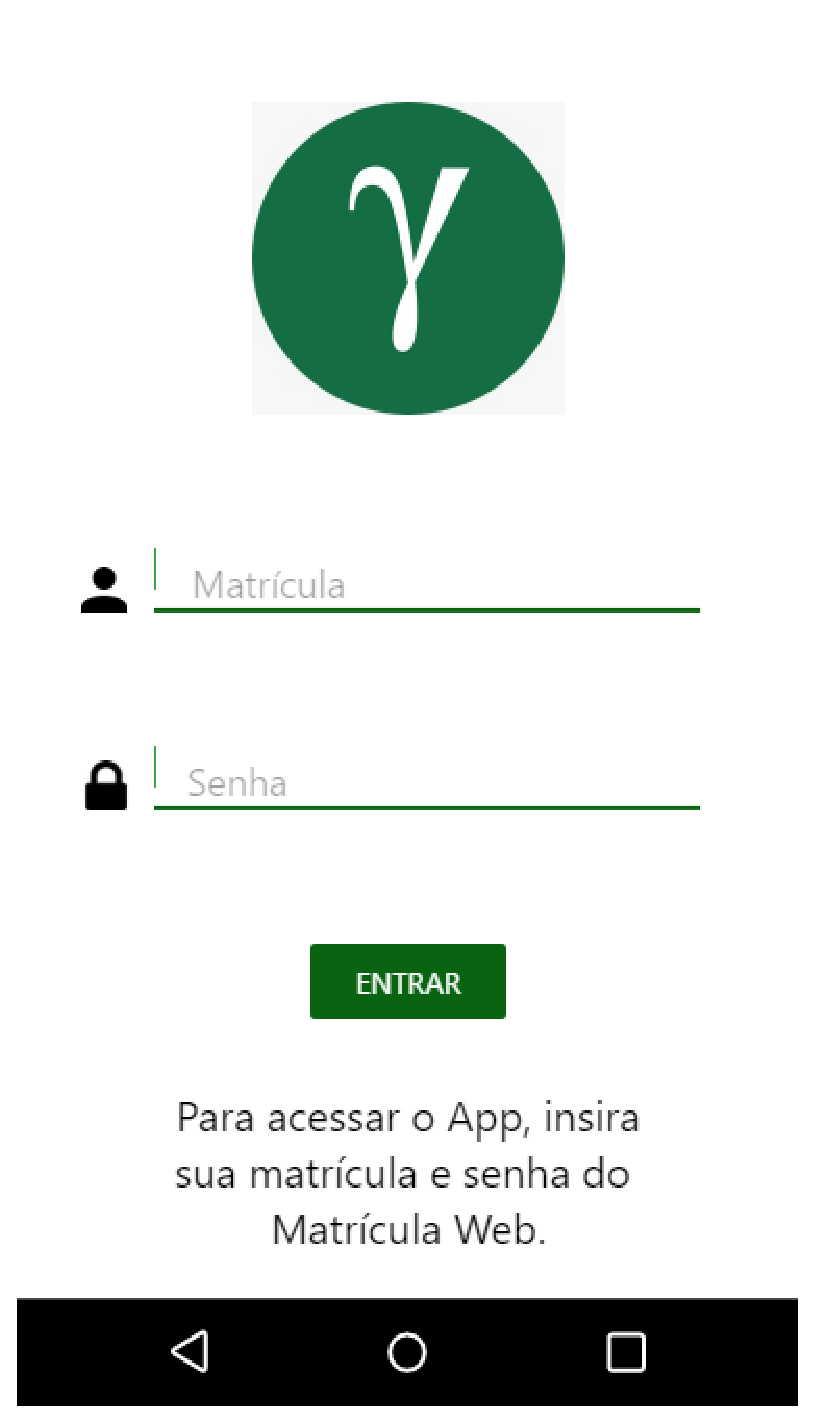
\includegraphics[keepaspectratio=true,scale=0.6]{figuras/prot-0.eps}
  \caption{Protótipo do Aplicativo - Parte 1}
\end{figure}

\begin{figure}[!h]
  \centering
  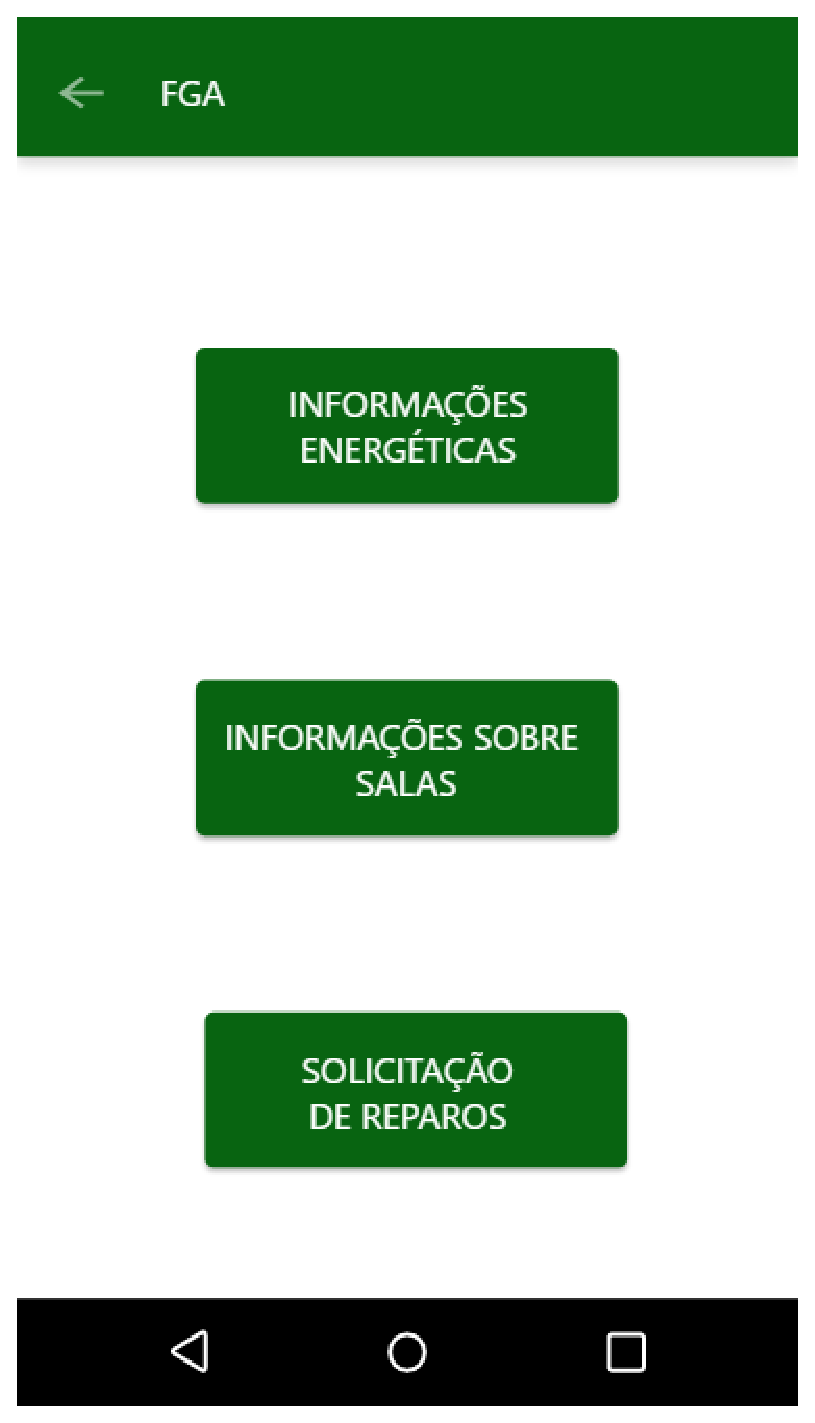
\includegraphics[keepaspectratio=true,scale=0.6]{figuras/prot-1.eps}
  \caption{Protótipo do Aplicativo - Parte 2}
\end{figure}

\begin{figure}[!h]
  \centering
  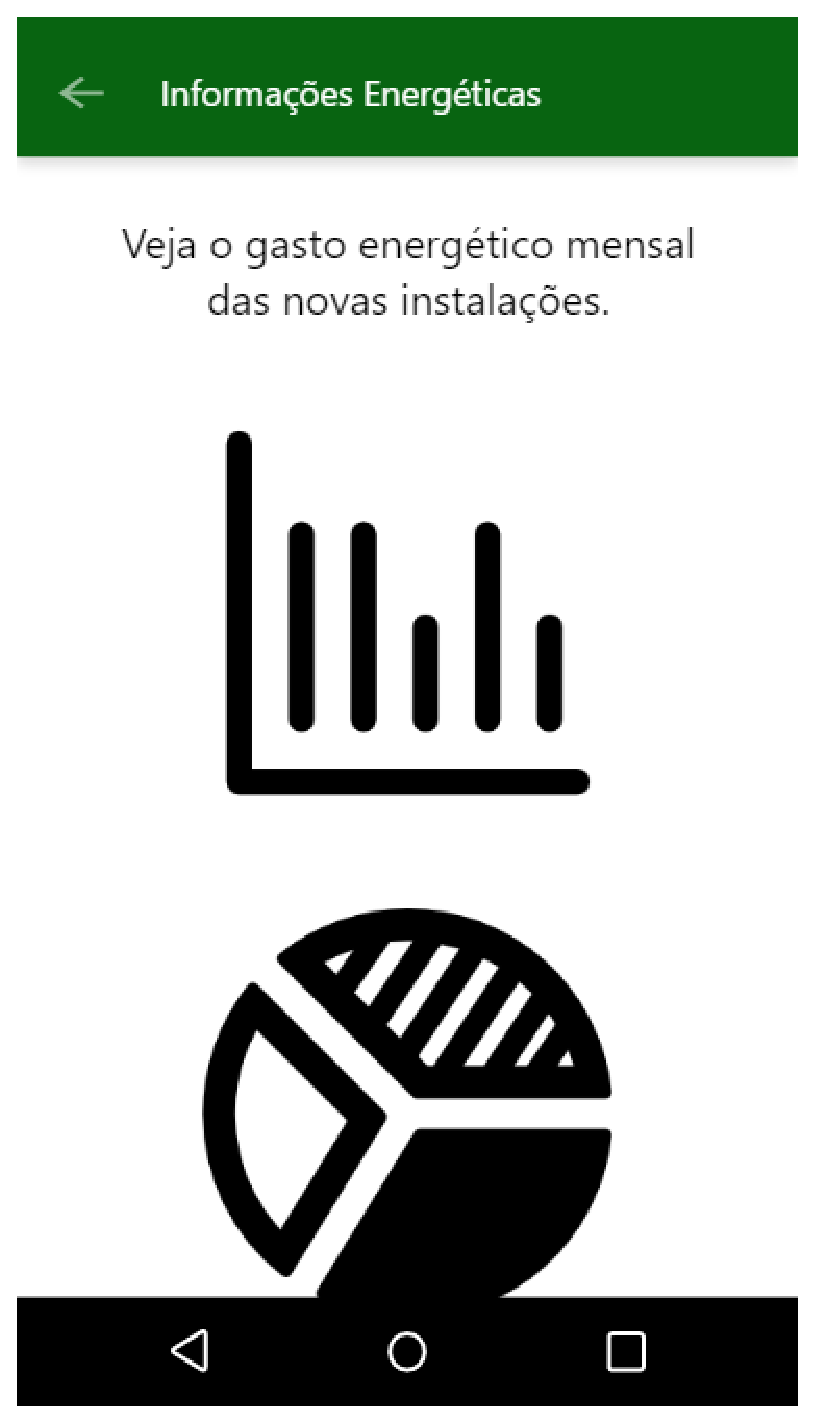
\includegraphics[keepaspectratio=true,scale=0.6]{figuras/prot-2.eps}
  \caption{Protótipo do Aplicativo - Parte 3}
\end{figure}

\begin{figure}[!h]
  \centering
  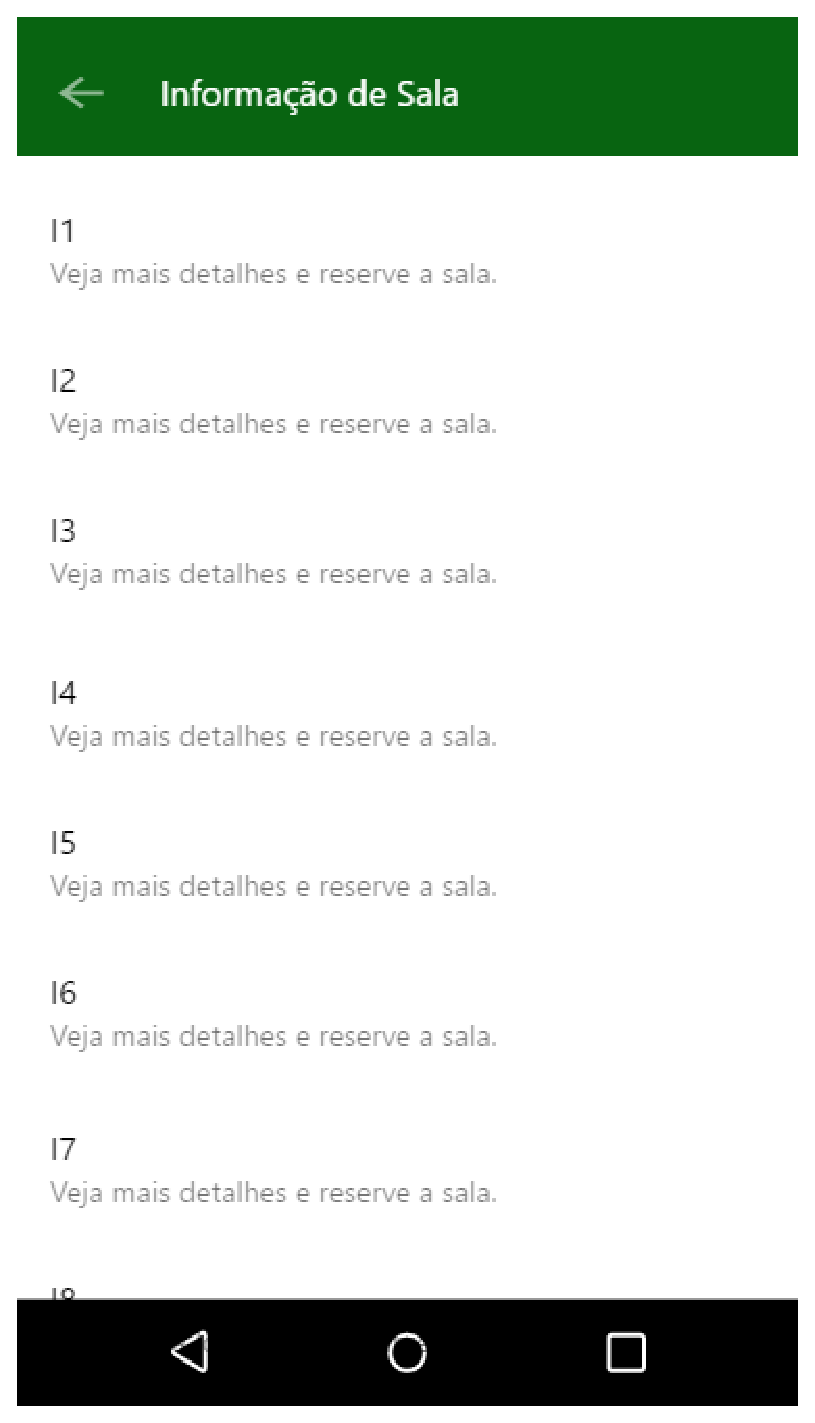
\includegraphics[keepaspectratio=true,scale=0.6]{figuras/prot-3.eps}
  \caption{Protótipo do Aplicativo - Parte 4}
\end{figure}

\begin{figure}[!h]
  \centering
  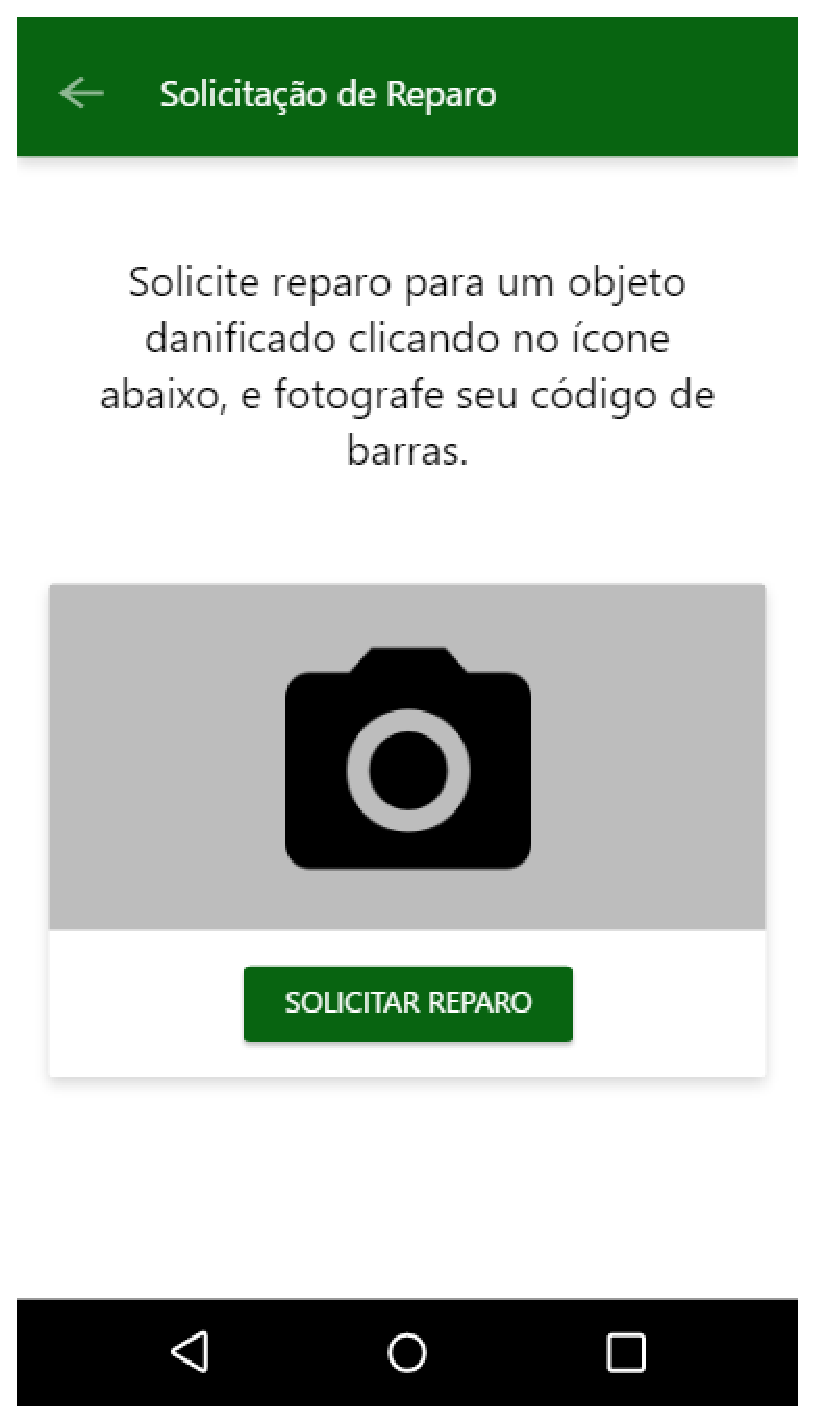
\includegraphics[keepaspectratio=true,scale=0.6]{figuras/prot-4.eps}
  \caption{Protótipo do Aplicativo - Parte 5}
\end{figure}

\begin{figure}[!h]
  \centering
  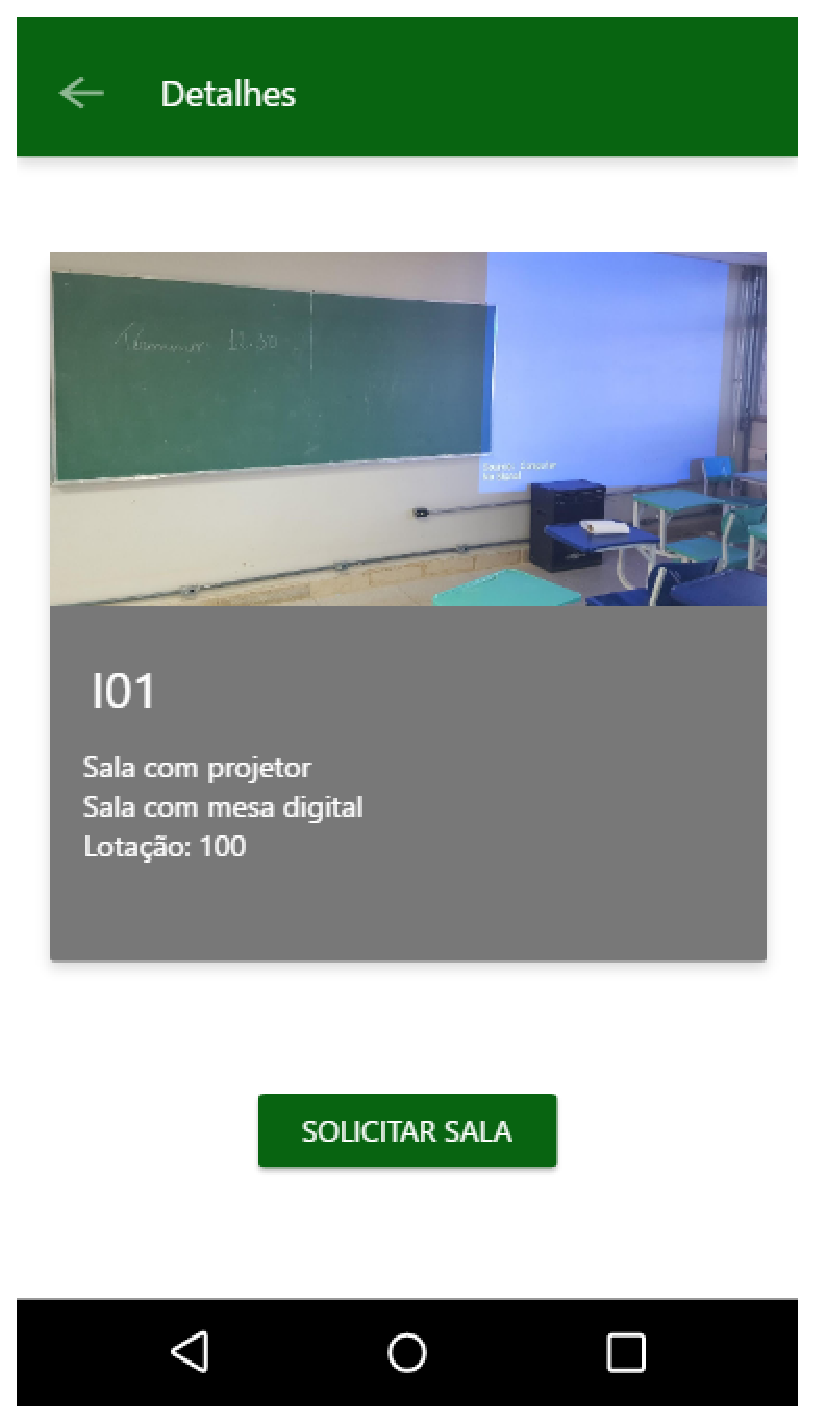
\includegraphics[keepaspectratio=true,scale=0.6]{figuras/prot-5.eps}
  \caption{Protótipo do Aplicativo - Parte 6}
\end{figure}

% \chapter{Segundo Anexo}
%
% Texto do segundo anexo.

\end{anexosenv}
